% (The MIT License)
%
% Copyright (c) 2023 Yegor Bugayenko
%
% Permission is hereby granted, free of charge, to any person obtaining a copy
% of this software and associated documentation files (the 'Software'), to deal
% in the Software without restriction, including without limitation the rights
% to use, copy, modify, merge, publish, distribute, sublicense, and/or sell
% copies of the Software, and to permit persons to whom the Software is
% furnished to do so, subject to the following conditions:
%
% The above copyright notice and this permission notice shall be included in all
% copies or substantial portions of the Software.
%
% THE SOFTWARE IS PROVIDED 'AS IS', WITHOUT WARRANTY OF ANY KIND, EXPRESS OR
% IMPLIED, INCLUDING BUT NOT LIMITED TO THE WARRANTIES OF MERCHANTABILITY,
% FITNESS FOR A PARTICULAR PURPOSE AND NONINFRINGEMENT. IN NO EVENT SHALL THE
% AUTHORS OR COPYRIGHT HOLDERS BE LIABLE FOR ANY CLAIM, DAMAGES OR OTHER
% LIABILITY, WHETHER IN AN ACTION OF CONTRACT, TORT OR OTHERWISE, ARISING FROM,
% OUT OF OR IN CONNECTION WITH THE SOFTWARE OR THE USE OR OTHER DEALINGS IN THE
% SOFTWARE.

\documentclass{article}
\usepackage{../sqm}
\usepackage{amsmath}
\usepackage{relsize}
\newcommand*\thetitle{Code Duplication}
\begin{document}

\plush{\sqmTitlePage{11}}

\pptBanner{Motivating Example}
\begin{multicols}{2}
Before (\textcolor{red}{wrong}):\par
{\small\begin{ffcode}
printf("Hi, %s!", getName(42));
printf("Hi, %s!", getName(7));
printf("Hi, %s!", getName(55));
\end{ffcode}
}
\par\columnbreak\par
After (\textcolor{green}{right}):\par
{\small\begin{ffcode}
sayHello(42);
sayHello(7);
sayHello(556);

void sayHello(int id) {
  var n = getName(id);
  printf("Hi, %s!", n);
}
\end{ffcode}
}
\end{multicols}
\plush{}

\pitch{\pptQuote{brenda-baker.jpg}{Two lines of code are considered to be identical if they contain the same \emph{sequence of characters} after removing comments and white space; the \emph{semantics} of the program statements are not analyzed.}{\textit{A Program for Identifying Duplicated Code}, Brenda S. Baker, Computing Science and Statistics, 1993}}

\pptBanner{Up to 38\% of lines are involved in duplicates}
\begin{multicols}{2}
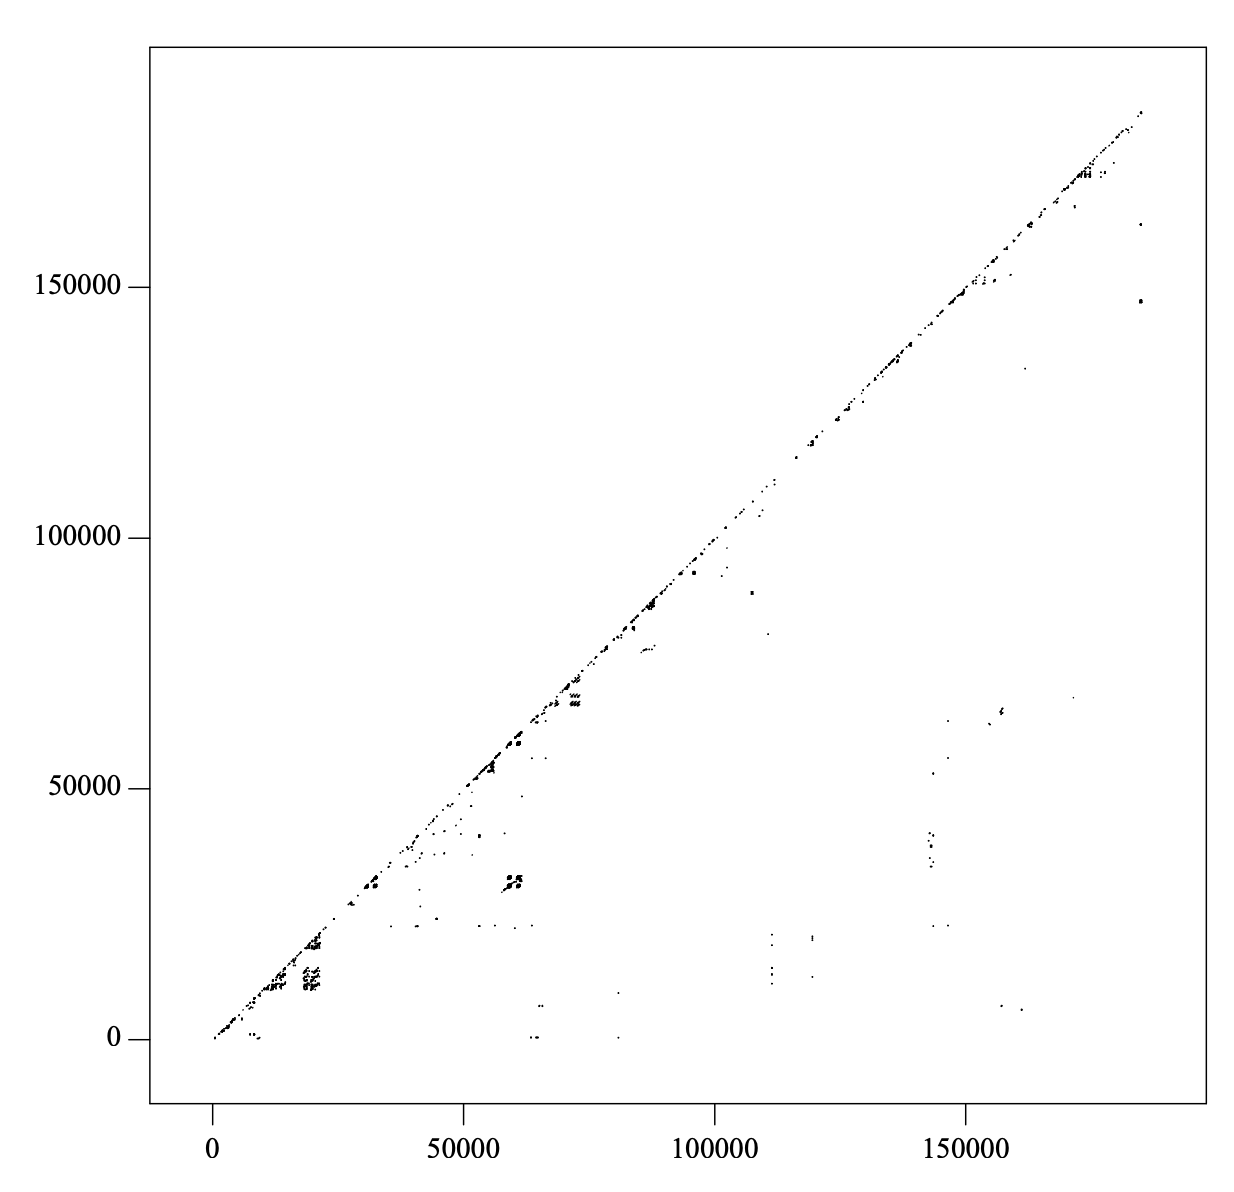
\includegraphics[width=.9\columnwidth]{scatter.png}
\par\columnbreak\par
The plots are dense near the main diagonal, implying
that most copies tend to occur \emph{fairly locally}, e.g. within the
same file or module. \par However, certain line segments occur
away from the main diagonal; it would be interesting to
investigate why the corresponding sections of code are
duplicated.
\end{multicols}
\plush{}

\pitch{\pptBanner{Don't Repeat Yourself (DRY)}\pptQuote{andy-hunt.jpg}{Every piece of knowledge must have a \emph{single}, unambiguous, authoritative representation within a system.}{\textit{The Pragmatic Programmer: From Journeyman to Master}, \emph{Andrew Hunt} and David Thomas, Addison-Wesley, 1999}}

\pitch{\pptBanner{The Rule of Three}\pptQuote{kent-beck.jpg}{The \emph{first} time you do something, you just do it. The \emph{second} time you do something similar, you wince at the duplication, but you do the duplicate thing anyway. The \emph{third} time you do something similar, you refactor.}{\textit{Refactoring}, Martin Fowler and \emph{Kent Beck}, Addison-Wesley, 1999}}


\plush{
  \pptBanner{These tools can help detecting duplicate code:}
  \begin{enumerate}
    \item ...
  \end{enumerate}
}

\plush{
  \pptBanner{Read this:}\par
  \small
  \textit{A Program for Identifying Duplicated Code},
    Brenda S. Baker,
    Computing Science and Statistics, 1993\par
  \textit{The Pragmatic Programmer: From Journeyman to Master},
     Andrew Hunt and David Thomas,
     Addison-Wesley, 1999
  \textit{Refactoring},
     Martin Fowler and Kent Beck,
     Addison-Wesley, 1999
}

\end{document}
